%% using aastex version 6.2
\documentclass[RNAAS]{aastex62}

%% The default is a single spaced, 10 point font, single spaced article.
%% There are 5 other style options available via an optional argument. They
%% can be envoked like this:
%%
%% \documentclass[argument]{aastex62}
%% 
%% where the layout options are:
%%
%%  twocolumn   : two text columns, 10 point font, single spaced article.
%%                This is the most compact and represent the final published
%%                derived PDF copy of the accepted manuscript from the publisher
%%  manuscript  : one text column, 12 point font, double spaced article.
%%  preprint    : one text column, 12 point font, single spaced article.  
%%  preprint2   : two text columns, 12 point font, single spaced article.
%%  modern      : a stylish, single text column, 12 point font, article with
%% 		  wider left and right margins. This uses the Daniel
%% 		  Foreman-Mackey and David Hogg design.
%%  RNAAS       : Preferred style for Research Notes which are by design 
%%                lacking an abstract and brief. DO NOT use \begin{abstract}
%%                and \end{abstract} with this style.
%%
%% Note that you can submit to the AAS Journals in any of these 6 styles.
%%
%% There are other optional arguments one can envoke to allow other stylistic
%% actions. The available options are:
%%
%%  astrosymb    : Loads Astrosymb font and define \astrocommands. 
%%  tighten      : Makes baselineskip slightly smaller, only works with 
%%                 the twocolumn substyle.
%%  times        : uses times font instead of the default
%%  linenumbers  : turn on lineno package.
%%  trackchanges : required to see the revision mark up and print its output
%%  longauthor   : Do not use the more compressed footnote style (default) for 
%%                 the author/collaboration/affiliations. Instead print all
%%                 affiliation information after each name. Creates a much
%%                 long author list but may be desirable for short author papers
%%
%% these can be used in any combination, e.g.
%%
%% \documentclass[twocolumn,linenumbers,trackchanges]{aastex62}
%%
%% AASTeX v6.* now includes \hyperref support. While we have built in specific
%% defaults into the classfile you can manually override them with the
%% \hypersetup command. For example,
%%
%%\hypersetup{linkcolor=red,citecolor=green,filecolor=cyan,urlcolor=magenta}
%%
%% will change the color of the internal links to red, the links to the
%% bibliography to green, the file links to cyan, and the external links to
%% magenta. Additional information on \hyperref options can be found here:
%% https://www.tug.org/applications/hyperref/manual.html#x1-40003
%%
%% If you want to create your own macros, you can do so
%% using \newcommand. Your macros should appear before
%% the \begin{document} command.
%%
\newcommand{\vdag}{(v)^\dagger}
\newcommand\aastex{AAS\TeX}
\newcommand\latex{La\TeX}

\received{\today}
\revised{\today}
\accepted{\today}
\submitjournal{RNAAS}

\shorttitle{B1937+21 Giant Pulse}
\shortauthors{Foster and Karastergiou}

\begin{document}

\title{A Giant Pulse detected from B1937+21 during LOFAR-UK Observations}

\correspondingauthor{Griffin Foster}
\email{griffin.foster@physics.ox.ac.uk}

\author[0000-0002-7559-4291]{Griffin Foster}
\affil{University of Oxford, Sub-Department of Astrophysics \\
Denys Wilkinson Building, Keble Road \\
Oxford, OX1 3RH, United Kingdom}

\author{Aris Karastergiou}
\affil{University of Oxford, Sub-Department of Astrophysics \\
Denys Wilkinson Building, Keble Road \\
Oxford, OX1 3RH, United Kingdom}
\affil{Physics Department, University of the Western Cape\\
Cape Town 7535, South Africa}
\affil{Department of Physics and Electronics, Rhodes University\\
PO Box 94, Grahamstown 6140, South Africa}

\keywords{pulsars: individual B1937+21, scattering, radio continuum: general}

\section{}

A Giant Pulse (GP) from B1937+21 \citep{1982Natur.300..615B} was detected during
observations with the LOFAR-UK station using the  ARTEMIS
\citep{2015MNRAS.452.1254K} pulse detection back-end at 2016-06-20 01:46:32.457
UTC. The detection occurred using the high-band array (HBA) centred at 145~MHz
with a bandwidth of $5.85$~MHz. After initial detection the dynamic spectrum was
incoherently de-dispersed with a Dispersion Measure (DM) of $71.0237$~pc~cm$^{-3}$.
The time series of the pulse is shown in Figure \ref{fig:pulse}. The data is
time smoothed using a boxcar function to a resolution of $2.6$~ms.

The system equivalent flux density (SEFD) of an international station HBA is
measured to be approximately 1900~Jy over the observed region of the band
\footnote{https://www.astron.nl/radio-observatory/astronomers/lofar-imaging-capabilities-sensitivity/sensitivity-lofar-array/sensiti}.
Using the radiometer equation results in a system noise of approximately 14~Jy
at a time resolution of $2.6$~ms and bandwidth $5.8$~MHz. The scattered pulse has
a measured peak flux of approximately 131~Jy.

An isotropic scattering model \citep{2017MNRAS.470.2659G} was fit to the pulse
resulting in a fit scattering time scale $\tau$ of $3.2 \pm 0.3$~ms consistent
with the expected scattering using the NE2001 \citep{2002astro.ph..7156C} model of
$3.27$~ms. The fit for the pulse before scattering is unresolved in width and
has an flux of $270 \pm 34$~Jy.

The dynamic spectrum data and analysis notebook is available on
github\footnote{https://github.com/griffinfoster/B1937-21-GP-Note}.

% aslxlap07:~/local/data/LOFAR/B1937+21/B1937+21.ipynb
\begin{figure}
	\centering
    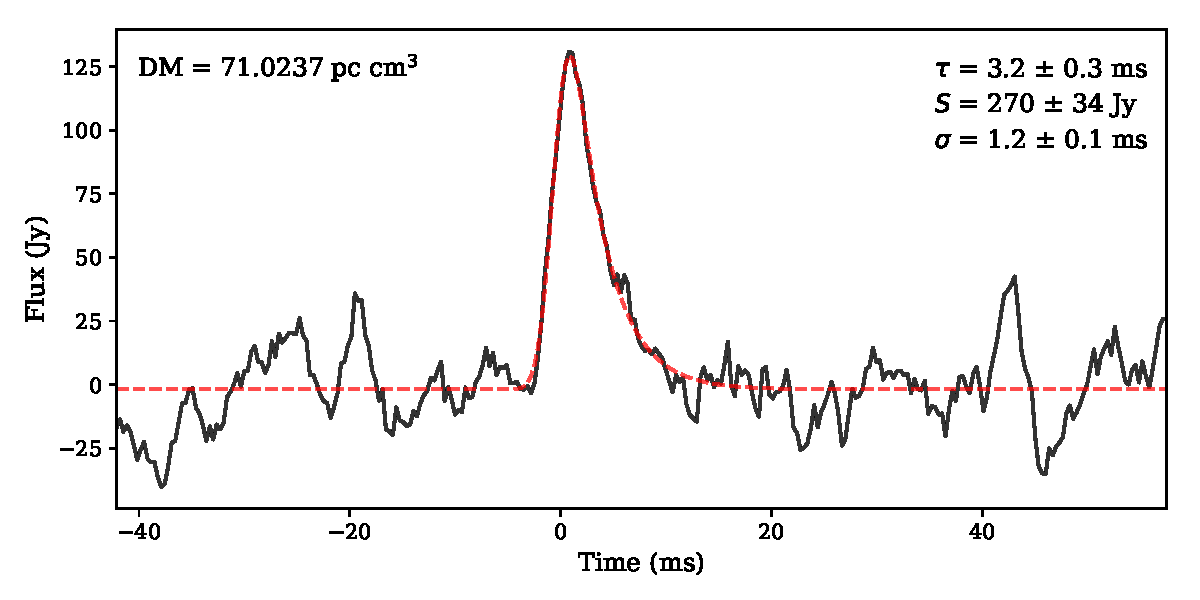
\includegraphics[width=0.75\linewidth]{figures/B1937+21_pulse.pdf}
    \caption{Time series of a giant pulse from B1937+21 (black solid), the data
    has been smoothed with a boxcar filter to a time resolution of $2.6$~ms. An
    isotropic scattering model has been fit to the pulse (red dashed). The best fit
    model parameters are presented in the upper right corner.
    }
    \label{fig:pulse}
\end{figure}

\bibliographystyle{aasjournal}
\bibliography{refs}

\end{document}
